\documentclass{article}

\usepackage[bookmarks]{hyperref}
\usepackage{fancyhdr} % Required for custom headers
\usepackage{lastpage} % Required to determine the last page for the footer
\usepackage{extramarks} % Required for headers and footers
\usepackage[usenames,dvipsnames]{color} % Required for custom colors
\usepackage{graphicx} % Required to insert images
\usepackage{listings} % Required for insertion of code
\usepackage{courier} % Required for the courier font
\usepackage{lipsum} % Used for inserting dummy 'Lorem ipsum' text into the template

% Margins
\topmargin=-0.45in
\evensidemargin=0in
\oddsidemargin=0in
\textwidth=6.5in
\textheight=9.0in
\headsep=0.25in

\linespread{1.1} % Line spacing

% Set up the header and footer
\pagestyle{fancy}
\lhead{} % Top left header
\chead{\hmwkProject: \hmwkTitle} % Top center head
\rhead{\firstxmark} % Top right header
\lfoot{\lastxmark} % Bottom left footer
\cfoot{} % Bottom center footer
\rfoot{Page\ \thepage\ of\ \protect\pageref{LastPage}} % Bottom right footer
\renewcommand\headrulewidth{0.4pt} % Size of the header rule
\renewcommand\footrulewidth{0.4pt} % Size of the footer rule

\setlength\parindent{0pt} % Removes all indentation from paragraphs

%----------------------------------------------------------------------------------------
%	CODE INCLUSION CONFIGURATION
%----------------------------------------------------------------------------------------
\definecolor{MyDarkGreen}{rgb}{0.0,0.4,0.0} % This is the color used for comments
\lstloadlanguages{C} % Load Perl syntax for listings, for a list of other languages supported see: ftp://ftp.tex.ac.uk/tex-archive/macros/latex/contrib/listings/listings.pdf
\lstset{language=C, % Use C in this example
        frame=single, % Single frame around code
        basicstyle=\small\ttfamily, % Use small true type font
        keywordstyle=[1]\color{Blue}\bf, % Perl functions bold and blue
        keywordstyle=[2]\color{Purple}, % Perl function arguments purple
        keywordstyle=[3]\color{Blue}\underbar, % Custom functions underlined and blue
        identifierstyle=, % Nothing special about identifiers
        commentstyle=\usefont{T1}{pcr}{m}{sl}\color{MyDarkGreen}\small, % Comments small dark green courier font
        stringstyle=\color{Purple}, % Strings are purple
        showstringspaces=false, % Don't put marks in string spaces
        tabsize=5, % 5 spaces per tab
        %
        % Put standard Perl functions not included in the default language here
        morekeywords={@new, @delete, @ctor, @dtor},
        %
        % Put Perl function parameters here
        morekeywords=[2]{@namespace, @implementation, @definition, @class},
        %
        % Put user defined functions here
        morekeywords=[3]{@import},
       	%
        morecomment=[l][\color{Blue}]{...}, % Line continuation (...) like blue comment
        numbers=left, % Line numbers on left
        firstnumber=1, % Line numbers start with line 1
        numberstyle=\tiny\color{Blue}, % Line numbers are blue and small
        stepnumber=5 % Line numbers go in steps of 5
}

% Creates a new command to include a perl script, the first parameter is the filename of the script (without .pl), the second parameter is the caption
\newcommand{\KoocCode}[2]{
  \begin{itemize}
  \item[]\lstinputlisting[caption=#2,label=#1]{#1.kc}
  \end{itemize}
}
\newcommand{\KoocHeader}[2]{
  \begin{itemize}
  \item[]\lstinputlisting[caption=#2,label=#1]{#1.kh}
  \end{itemize}
}

\newcommand{\CCode}[2]{
  \begin{itemize}
  \item[]\lstinputlisting[caption=#2,label=#1]{#1.c}
  \end{itemize}
}
\newcommand{\CHeader}[2]{
  \begin{itemize}
  \item[]\lstinputlisting[caption=#2,label=#1]{#1.h}
  \end{itemize}
}

%----------------------------------------------------------------------------------------
%	DOCUMENT STRUCTURE COMMANDS
%	Skip this unless you know what you're doing
%----------------------------------------------------------------------------------------

%HyperRef Settings
\hypersetup{pdftex,colorlinks=true, allcolors=black}

% Header and footer for when a page split occurs within a problem environment
\newcommand{\enterFeature}[1] {
  \nobreak\extramarks{#1}{#1}\nobreak
  \nobreak\extramarks{#1}{#1}\nobreak
}

% Header and footer for when a page split occurs between problem environments
\newcommand{\exitFeature}[1]{
  \nobreak\extramarks{#1}{#1}\nobreak
  \nobreak\extramarks{#1}{}\nobreak
}

\setcounter{secnumdepth}{0} % Removes default section numbers
\newcounter{FeatureCounter} % Creates a counter to keep track of the number of problems

\newcommand{\FeatureName}{}
\newenvironment{Feature}[1][Problem \arabic{FeatureCounter}]{ % Makes a new environment called homeworkProblem which takes 1 argument (custom name) but the default is "Problem #"
  \stepcounter{FeatureCounter} % Increase counter for number of problems
  \renewcommand{\FeatureName}{#1} % Assign \homeworkProblemName the name of the problem

  \section{\FeatureName} % Make a section in the document with the custom problem count
  \enterFeature{\FeatureName} % Header and footer within the environment
}{
  \exitFeature{\FeatureName} % Header and footer after the environment
}

\newcommand{\FeatureSectionName}{}
\newenvironment{FeatureSection}[1][Test]{ % New environment for sections within homework problems, takes 1 argument - the name of the section
  \renewcommand{\FeatureSectionName}{#1} % Assign \homeworkSectionName to the name of the section from the environment argument
  \subsection{\FeatureSectionName} % Make a subsection with the custom name of the subsection
  \enterFeature{\FeatureName\ [\FeatureSectionName]} % Header and footer within the environment
}{
  \enterFeature{\FeatureName} % Header and footer after the environment
}

%----------------------------------------------------------------------------------------
%	NAME AND CLASS SECTION
%----------------------------------------------------------------------------------------

\newcommand{\hmwkTitle}{Conception} % Assignment title
\newcommand{\hmwkProject}{Kooc} % Course/class
\newcommand{\hmwkAuthorName}{Colliot Vincent, Diego Moran, Frederic Lavrut} % Your name

%----------------------------------------------------------------------------------------
%	TITLE PAGE
%----------------------------------------------------------------------------------------

\title{
  \vspace{2in}
  \textmd{\textbf{\hmwkProject:\ \hmwkTitle}}\\
  \vspace{3in}
}

\author{\textbf{\hmwkAuthorName}}
\date{} % Insert date here if you want it to appear below your name

%----------------------------------------------------------------------------------------

\begin{document}

\maketitle

%----------------------------------------------------------------------------------------
%	TABLE OF CONTENTS
%----------------------------------------------------------------------------------------

%\setcounter{tocdepth}{1} % Uncomment this line if you don't want subsections listed in the ToC

\newpage
\tableofcontents
\newpage

%----------------------------------------------------------------------------------------
%       Kooc
%----------------------------------------------------------------------------------------

\begin{Feature}[Kooc]
  \begin{FeatureSection}[What]
    The Kooc is an Epitech project. It's purpose is to design an Object Oriented Language, and create a compiler able to compile our language, and translate it into functional C. \newline
  \end{FeatureSection}
  \begin{FeatureSection}[Technologies]
    The compiler will be written in Python. It will use the modules Pyrser (to parse the language) and Cnorm (to parse C, and digest our code into C). \newline
  \end{FeatureSection}
  \begin{FeatureSection}[Implementation]
    The compiler will work in two steps : \newline
    * First, it will parse the file, recursively including any needed files (\.kh) precised by an \@ import directive. This file will construct what we call an Abstract Syntax Tree (AST) accord to the parsing rules. This AST is made of multiples layers of Nodes, each with its own definition, properties and datas. Since the compiler is able to parse both a pure C code, and a mixed C/KOOC code, we decided by design to add our own parsing rules and nodes (as to avoid collisions with Cnorm) on top of Cnorm. \newline
    * Second, we will recursively go through our AST : if a C node is found, it is processed according to Cnorm. But if one of our own nodes is found, it will then be resolved according to our own methods, and translated into an appropriate block of C nodes. The Kooc node is then removed from the AST. \newline
  \end{FeatureSection}
  \begin{FeatureSection}[Implemented]
    As of now, what is currently implemented ? \newline \newline


    We have a functional mangler, import, namespaces, classes with linear and multiple inheritances. \newline
    We thought about type inference, polymorphism, exceptions, but these are, at best, only partly implemented. \newline
    These will be explained below. \newline
    We also dispose of a robust error management : forbid implementation when the previous definition is lacking, manage attributes and methods visibilities, nesting errors, missing constructors or destructors in a class. \newline
  \end{FeatureSection}
\end{Feature}
\clearpage

%----------------------------------------------------------------------------------------
%       Mangling
%----------------------------------------------------------------------------------------

\begin{Feature}[Mangling]
  \begin{FeatureSection}[What]
    Mangling/Name Mangling is a technique used to avoid many problem on unique names resolution. \newline
    Mangling will modify the name following some pattern in order to avoid name collisions. \newline
  \end{FeatureSection}
  \begin{FeatureSection}[Why]
      We needed to solve unique name resolution to be able to create a C oriented object. \newline
      When you create a Class in cpp you're going to set variables and methods in it, if we want to simulate this we need to tell in C that a function is only callable by the object. \newline
      The solution for this is to change the function name to className\_functionName. \newline
      The function can in fact still be called by the user. This is why we obfuscate the name : to reduce risks of collisions. \newline
  \end{FeatureSection}
  \begin{FeatureSection}[Code Equivalence]
    \KoocHeader{mangling}{ various examples in Kooc }
    \CHeader{mangling}{ various examples in C }
  \end{FeatureSection}
  \begin{FeatureSection}[Implementation]
    \_\_\_[\{nb\}NAMESPACE\_\_]*[\{nb\}CLASS\_\_]?\{nb\}SYMTYPE\_\_\{nb\}SYMNAME[\_\_[\{nb\}TYPARG\_\_]*\{nb\}RETTYPE]?\_\_ \newline
    \{nb\} = len(word) \newline
    When we mangle we add \_\_\_ as separator at the begining and \_\_ between informations, before all informations we tell the length of the information's string. \newline
    We mangle with all the namespaces, the class if present, and the type. Symtype makes the difference between a function or a variable. Symname is the name given to this symbol. \newline
    Then, if it's a function, we also mangle with every argument's type, and the return type. \newline
    This is implemented by a Class who have for purpose to change the variable name like the previous declaration. \newline
    To be noted : a mangling by type of arguments/type of the variable is implemented (for type inference purpose) but desactivated, as the functionality is not complete. \newline
  \end{FeatureSection}
  \begin{FeatureSection}[Note]
    Note : further examples will use \'\'MANGLED_\'\' instead of our real mangling, for the sake of lisibility. \newline
  \end{FeatureSection}
\end{Feature}
\clearpage

%----------------------------------------------------------------------------------------
%	Import
%----------------------------------------------------------------------------------------

\begin{Feature}[Import]
  \begin{FeatureSection}[What]
    To support the use of import in our kooc we use an @Import Statement for safe inclusion. \newline
  \end{FeatureSection}
  \begin{FeatureSection}[Why]
    We needed to be able to include header in our languague so we used @Import as statement to simulate the \#include.
  \end{FeatureSection}
  \begin{FeatureSection}[Code Equivalence]
    \KoocCode{import}{ Import demo in Kooc code }
    \CCode{import}{ Import translation in C code }
  \end{FeatureSection}
  \begin{FeatureSection}[Implementation]
    To implement this we created a custom node (Imp). When this node is found, we add it in our AST. \newline
    When resolving our newly created AST, for each Imp node encountered, we will replace it by a normal \#include, encapsulated by define/ifndef directives, and remove this node from the AST. \newline
  \end{FeatureSection}
\end{Feature}
\clearpage

%----------------------------------------------------------------------------------------
%	Namespace
%----------------------------------------------------------------------------------------

\begin{Feature}[Namespace]
  \begin{FeatureSection}[What]
    The purpose of a namespace is to define sub context for declaration of variables and functions. One of the common objective of namespace is to reduce the risk of naming collisions, and permit a new layer of logic isolation. \newline
  \end{FeatureSection}
  \begin{FeatureSection}[Why]
    To be able to use our languague as an object oriented languague we needed to add a Namespace declaration. \newline
  \end{FeatureSection}
  \begin{FeatureSection}[Code Equivalence]
    \KoocHeader{namespace}{ Namespace demo in Kooc header }
    \CHeader{namespace}{ Namespace translation in C header }
    \KoocCode{namespace}{ Namespace demo in Kooc code }
    \CCode{namespace}{ Namespace translation in C code }
  \end{FeatureSection}
  \begin{FeatureSection}[Implementation]
    The definition of a namespace (called 'module' in the subject) is @namespace(NAME)\{\}, and its implementation is @definition(NAME)\{\} \newline
    We implemented this by detecting Namespace declaration (@definition) and added a node in our AST. \newline
    When encountered, this node tells us to do all the mangling and operation of transformation for a Namespace declaration. We then remove this node from the AST. \newline
    As of now, nested namespaces is possible and functional. \newline
  \end{FeatureSection}
\end{Feature}
\clearpage

%----------------------------------------------------------------------------------------
%	Class
%----------------------------------------------------------------------------------------

\begin{Feature}[Class]
  \begin{FeatureSection}[What]
    A class is an object containing variables and methods. Linear and Multiple Inheritance is a possibility of classes. \newline
  \end{FeatureSection}
  \begin{FeatureSection}[Why]
    To be able to use our languague as an object oriented languague we needed to add a Class declaration. \newline
  \end{FeatureSection}
  \begin{FeatureSection}[Code Equivalence]
    \KoocHeader{class}{ Class demo in Kooc header }
    %% \CHeader{class}{ Class translation in C header }
    \KoocCode{class}{ Class demo in Kooc code }
    %% \CCode{class}{ Class translation in C code }
  \end{FeatureSection}
  \begin{FeatureSection}[Implementation]
    The definition of a class is @class(NAME)\{\}, and its implementation is @implementation(NAME)\{\} \newline
    Like the previous implementation of Namespace, we created a node to do the specific mangling and transformation of the code. \newline
    Methods can be private or public and can be set to virtual or override. Attributes can be set private, public or public. This will be explained below. \newline
  \end{FeatureSection}
\end{Feature}
\clearpage

%----------------------------------------------------------------------------------------
%	Properties, Visibilities
%----------------------------------------------------------------------------------------

\begin{Feature}[Properties and Visibilities]
  \begin{FeatureSection}[What]
    In our class, we can add properties to methods and visibilities to both methods and attributes. \newline
  \end{FeatureSection}
  \begin{FeatureSection}[Why]
    Those properties and visibilities are key to both respect encapsulation and virtuality, key principles in an object oriented language. \newline
  \end{FeatureSection}
  \begin{FeatureSection}[Implementation]
    Those additionals informations are added inside our class nodes, used in the resolve process (to verify if a future use isn\'t forbidden), and then removed along the node. \newline
    For visibility, you can set it to public (everyone can use it), protected (only classes inheriting it can use it), or private (only the current class can use it). Visibility can be applied to methods and attributes.
    For inheritance properties, you can set it to none (a normal method), virtual (say than this method will be overrided), or override (this override a parent class\' method precised as virtual). \newline
  \end{FeatureSection}
\end{Feature}
\clearpage

%----------------------------------------------------------------------------------------
%	Linear And Multi Inheritance
%----------------------------------------------------------------------------------------

\begin{Feature}[Linear and Multi Inheritance]
  \begin{FeatureSection}[What]
    Inheritance is the principle of extending a \'\'Child class\'\' with the methods and attributes of a \'\'Parent class\'\', and then manipulate a Child class as you would manipulate a Parent class. \newline
    Linear Inheritance is when your object have one Parent maximum. \newline
    Multi Inheritance is when your object have more than one Parent. In this case, some problems appear. The most infamous problem is the \'\'Diamond\'\', where your child class A inherit from both classes B and C, and both of them inherit from the same class D : How to know which methods to use ? \newline
  \end{FeatureSection}
  \begin{FeatureSection}[Research]
    We haved researched a lot of differents implementations of what we consider multi Inheritance. \newline
    Since our implementation is based on C++, we will explain it below. \newline
    In Python, it is done by linearizing the inheritance : When a Child class A inherits from classes B, C and D simultaneously, Python creates temporary classes : tmpC inherited from D, tmpB inherited from tmpC, and A inherited from tmpB. To do so, it will call the MRO Algorithm, resolving both parent inheritances in B, C and D and forbid Diamonds. Since we don\'t have polymorphism, using a Python-like multi inheritance is impossible. Typically in Python, if a class inherit from B, C and D (and all of them implements a Foo method), and because you inherit from D, then from C, then from B, when you call Foo, you will use Foo of B.\newline
    In some languages, parent classes are replaced by Mixins, or Traits. Classes will \'\'include\'\' Mixins\' code, rather than \'\'inherit from it\'\'. Mixins can be seen as interfaces containing implemented methods : it doesnt have an identity by itself, and as such a child class \'\'including\'\' code from a Mixin CANT be used as a Mixin instance, since a Mixin has no instance. Traits and Mixins are different only in the way of handling multi inheritances : Mixins explicitly forbid it, where Traits have ways to implement it (depends on the language). We didnt implement Mixins nor Traits because both us and the subject judged it as too restrictive.\newline
  \end{FeatureSection}
  \begin{FeatureSection}[Implementation]
    We decided to implement a C++-like inheritance, where we copy all the attributes and methods from the parent(s) into the child class. \newline
    Like C++, we also manage a Virtual Table. This will be explained below. \newline
    With our implementation, a Diamond problem will output an error (because both class inheriting from the same class will contain the same attributes, and we don\'t manage it) OR use the method from the first inherited class in our child class (when there is no attributes conflicts, and because we search for the first valid implementation of asked class). \newline
    Unlike some languages (Java, ...) we don\'t have an \'\'Origin\'\' class, which is inherited by all existing objects. \newline
  \end{FeatureSection}
\end{Feature}
\clearpage

%----------------------------------------------------------------------------------------
%	Vtable
%----------------------------------------------------------------------------------------

\begin{Feature}[Vtable]
  \begin{FeatureSection}[What]
    A Vtable is a virtual table where all pointer virtual methods are stored to be able to use them in our subclass. \newline
  \end{FeatureSection}
  \begin{FeatureSection}[Why]
    Whenever a class inherit from an another class we need to have the virtual table of this class. \newline
    To support inheritance we need to be able to use virtual methods of the inherited class. \newline
    With inheritance and virtual method we can create a complex code with less lines by avoiding code reuse. \newline
  \end{FeatureSection}
  \begin{FeatureSection}[Code Equivalence]
    \KoocHeader{simpleVtable}{ Simple Inheritance demo in Kooc header }
    \CHeader{simpleVtable} { Simple Inheritance demo in c header }
    \KoocCode{simpleVtable}{ Simple Inheritance demo in Kooc code }
    \CCode{simpleVtable}{ Simple Inheritance demo in c code }
    \KoocHeader{complexVtable}{ Multiple Inheritance demo in Kooc header }
    \CHeader{complexVtable} { Multiple Inheritance demo in C header }
    \KoocCode{complexVtable}{ Multiple Inheritance demo in Kooc code }
    \CCode{complexVtable}{ Multiple Inheritance demo in c code }
  \end{FeatureSection}
  \begin{FeatureSection}[Implementation]
    How we did it in memory for simple inheritance (@class b(a)) \newline
    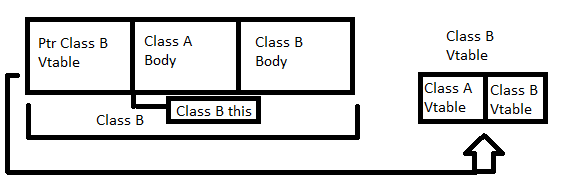
\includegraphics{simplevtable} \newline
    How we did it in memory for multiple inheritance (@class ab(a,b)) \newline
    \includegraphics{multivtable} \newline
    We implemented the vtable by allocating 8 Bytes before the class to store a pointer of a pointer on the vtable. \newline
    In simple inheritance we add the vtable of the inherited class to the class who inherit it. \newline
    In multiple inheritance we add the first class' vtable to the child class' vtable and the others class' vtable are added before their body.\newline
  \end{FeatureSection}
\end{Feature}
\clearpage

%----------------------------------------------------------------------------------------
%       Exception
%----------------------------------------------------------------------------------------

\begin{Feature}[Exception]
  \begin{FeatureSection}[What]
    An exception is meant to change the standard flow of the process in case where something went wrong.
  \end{FeatureSection}
  \begin{FeatureSection}[Why]
    Use exception to raise an error is useful when something unexpected occured and you want to do something if this exception occured.
  \end{FeatureSection}
  \begin{FeatureSection}[Code Equivalence]
    \KoocCode{exception}{ Exception demo in Kooc code }
  \end{FeatureSection}
  \begin{FeatureSection}[Implementation]
    The definition of an exception is @throw(FUNCTION*)(VAR), and you can verify if an exception occured with @try\{\}. If an exception occured you may want to catch it with @catch(FUNCTION*)\{\}
    We tried to implement it but time was short so we dropped it to implement major functionality.
  \end{FeatureSection}
\end{Feature}
\clearpage

\end{document}
